\documentclass[letterpaper,12pt,fleqn]{article}
\usepackage{matharticle}
\usepackage{mathtools}
\usepackage{tikz}
\pagestyle{plain}
\begin{document}

\begin{center}
\Large Math-19 Homework \#1 Solutions
\end{center}

\vspace{0.5in}

\underline{Reading}

Please read sections 1.1 through 1.5 and do all concept problems in the posted
sections on web\-assign. This written homework is based on section 1.1 material
only.

\underline{Problems}

\begin{enumerate}
\item Let:
\begin{eqnarray*}
P &\coloneqq& 0\ \mbox{is a positive number} \\
Q &\coloneqq& 2\ge2 \\
R &\coloneqq& \forall n,m\in\mathbb{N}, n+m\in\mathbb{N} \\
\end{eqnarray*}
Determine whether the following compound statement is true or false:

\hspace{0.5in}P and Q and R or P and not Q and R or not P and Q and R

Start by rewriting the statement with parentheses to show operation order,
then substitute the truth value for each individual statement, and then
show the stepwise evaluation to the final result.

\bigskip

P is false. 0 is neither positive or negative.

Q is true. $2\le2$ means $2<2$ \emph{or} $2=2$. Since $2=2$ (reflexive
property) and since only one of the two statements has to be true, Q is true.

R is true. It is the statement of closure of addition on the natural numbers.

\hspace{0.5in}(P and Q and R) or (P and (not Q) and R) or ((not P) and Q and R)

\hspace{0.5in}(F and T and T) or (F and (not T) and T) or ((not F) and T and T)

\hspace{0.5in}F or (F and F and T) or (T and T and T)

\hspace{0.5in}F or F or T

\hspace{0.5in}T

\bigskip

\item Convert $10.2\overline{45}$ to rational form.

\bigskip

\begin{eqnarray*}
x &=& 10.2\overline{45} \\
10x &=& 102.\overline{45} \\
1000x &=& 10245.\overline{45} \\
\\
990x &=& 10143 \\
x &=& \frac{10143}{990}=\frac{1127}{110} \\
\end{eqnarray*}

\bigskip

\item Let:
\begin{eqnarray*}
A &=& \mbox{the set of all positive real numbers} \\
B &=& \mbox{the set of real numbers between -3 (exclusive) and 3 (inclusive)} \\
\end{eqnarray*}
\begin{enumerate}
\item Graph each set on the real number line.
\item Represent each set using set-builder notation.
\item Represent each set using interval notation.
\item Graph $A\cup B$ and represent it in interval notation.
\item Graph $A\cap B$ and represent it in interval notation.
\item Graph $A-B$ and represent it in interval notation.
\end{enumerate}

\bigskip

\newcommand{\tick}[1]{\draw (#1,0.1) -- (#1,-0.1)}
\newcommand{\ocirc}[1]{\draw (#1,0) circle [radius=0.1]}
\newcommand{\ccirc}[1]{\draw [fill=black] (#1,0) circle [radius=0.1]}

\begin{enumerate}
\item Graphs:

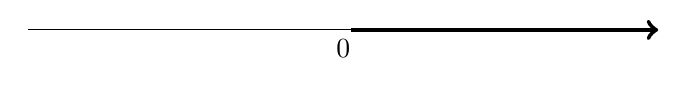
\begin{tikzpicture}
\draw (-4,0) -- (4,0);
\tick{0};
\ocirc{0};
\draw [->, ultra thick] (0.1,0) -- (4,0);
\node [below] at (0,0) {0};
\end{tikzpicture}

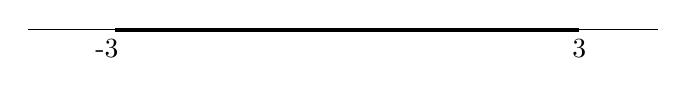
\begin{tikzpicture}
\draw (-4,0) -- (4,0);
\tick{-3};
\tick{3};
\ocirc{-3};
\ccirc{3};
\draw [ultra thick] (-2.9,0) -- (3,0);
\node [below] at (-3,0) {-3};
\node [below] at (3,0) {3};
\end{tikzpicture}

\item Setbuilder notation:
\[A=\{x\in\R\mid x>0\}\]
\[B=\{x\in\R\mid -3<x\le3\}\]

\item Interval notation:
\[A=(0,\infty)\]
\[B=(-3,3]\]

\item $A\cup B=(-3,\infty)$

\item $A\cap B=(0,3]$

\item $A-B=(3,\infty)$

\end{enumerate}

\bigskip

\item A careful solution of $4(x+2)=11$ is given below. Give the rationale for
each step from the ten real number rules (AC,AA,A0,AI,MC,MA,M1,MI,LD,RD) and
the additional rules (SUB,LCAN,RCAN).

\begin{tabular}{ll}
$4(x+2)=11$ & \\
$4x+8=11$ & LD \\
$(4x+8)-8=11-8$ & CAN \\
$(4x+8)-8=3$ & SUB \\
$4x+(8-8)=3$ & AA \\
$4x+0=3$ & AI \\
$4x=3$ & A0 \\
$\frac{1}{4}(4x)=\frac{1}{4}(3)$ & CAN \\
$\frac{1}{4}(4x)=\frac{3}{4}$ & SUB \\
$(\frac{1}{4}4)x=\frac{3}{4}$ & MA \\
$1x=\frac{3}{4}$ & MI \\
$x=\frac{3}{4}$ & M1 \\
\end{tabular}

\item Give a careful proof of $|a-b|=|b-a|$. You will need to use one of the
distributive rules, the definition of absolute value, and some of the
properties in box at the top of page 9. Be sure to justify each step.

\bigskip

\begin{tabular}{ll}
$\abs{a-b}=\abs{-(b-a)}$ & Prop of Neg \#6 \\
$\abs{a-b}=\abs{(-1)(b-a)}$ & Prop of Neg \#1 \\
$\abs{a-b}=\abs{-1}\abs{b-a}$ & Prop of AV \#3 \\
$\abs{a-b}=1\cdot\abs{b-a}$ & Def of AV \\
$\abs{a-b}=\abs{b-a}$ & M1 \\
\end{tabular}
\end{enumerate}
\end{document}
